\documentclass[a4paper,12pt]{article}
\usepackage[utf8]{inputenc}
\usepackage[spanish]{babel}
\usepackage{graphicx}
\graphicspath{{./figuras/}}
\usepackage[a4paper, left=2cm, right=2cm, top=2.5cm, bottom=2.5cm]{geometry}
\usepackage{xcolor} % Añadido para usar colores
\usepackage{amsmath}

% Definir un color para los títulos (puedes ajustar el color como quieras)
\definecolor{azulUPP}{RGB}{0,70,128} % Un azul corporativo o tecnológico

% Redefinir el formato de las secciones y subsecciones para incluir color
\usepackage{titlesec}
\titleformat{\section}{\Large\bfseries\color{azulUPP}}{}{0em}{\MakeUppercase}[]
\titleformat{\subsection}{\large\bfseries\color{azulUPP}}{}{0em}{}[]
\titleformat{\subsubsection}{\bfseries\color{azulUPP}}{}{0em}{}[]

\begin{document}
	% Portada
	\begin{titlepage}
		\centering
		% Logos institucionales y nombre de la universidad
		
\includegraphics[width=0.25\textwidth]{logoUpp} \hspace{7cm} 
		
\includegraphics[width=0.25\textwidth]{logoSftw}
		\vspace{2cm}
		
		\Huge \textbf{Universidad Politécnica de Pachuca}\\
		\vspace{0.5cm}
		\Large Ingeniería en Software
		\vspace{1cm}
		
		% Titulo
		\Huge \textbf{Conceptos Teóricos - Proyecto de Tercer Parcial.}
		\vspace{1cm}
		
		% Información completa
		\Large \textbf{Materia:} Arquitectura de computadoras \\
		\Large \textbf{Docente:} Víctor Hainy\\
		\vspace{1cm}
		\Large \textbf{Alumno:} \\Peña Serrano José Abraham\\
		\vspace{1cm}
		\Large \textbf{Matricula:} \\2331123273\\
		\vspace{1cm}
		\Large \textbf{Grupo:} SFTW\_06\_01\\
		\vspace{1cm}
		\Large \textbf{Cuatrimestre:} Mayo - Agosto 2025
		
	\end{titlepage}
	
	\tableofcontents
	
	\newpage
	\section{Objetivo de aprendizaje}
	Describir el uso y funcionamiento de los microcontroladores, actuadores y sistemas embebido en sistemas reales aplicados.
	
	\section{Conceptos Teóricos}
	
	\subsection{Microcontroladores}
	\subsubsection{Definición}
	Un \textbf{microcontrolador} es un circuito integrado que incluye en un solo chip los elementos esenciales de un sistema informático: una unidad central de procesamiento (CPU), memoria (RAM y ROM/Flash) y periféricos de entrada/salida (E/S). A diferencia de los microprocesadores convencionales, los microcontroladores están diseñados para controlar dispositivos específicos o sistemas embebidos, realizando tareas concretas de manera automática y eficiente. Se encuentran en aplicaciones tan variadas como electrodomésticos, automóviles, sistemas de automatización industrial y dispositivos médicos.
	
	El microcontrolador es el “cerebro” de sistemas electrónicos autónomos, permitiendo la interacción con el entorno y la automatización de tareas específicas sin requerir la intervención continua de un usuario.
	
	\subsubsection{Tipos}
	Existen varios criterios para clasificar los microcontroladores, siendo los más comunes:
	
	\begin{itemize}
		\item \textbf{Por arquitectura:}
		\begin{itemize}
			\item \textit{Basados en arquitectura Harvard:} Separan físicamente la memoria de instrucciones y de datos (por ejemplo, la familia PIC).
			\item \textit{Basados en arquitectura Von Neumann:} Comparten el mismo bus para instrucciones y datos (como algunos modelos de 8051).
		\end{itemize}
		\item \textbf{Por tamaño de palabra (bits):}
		\begin{itemize}
			\item Microcontroladores de 8 bits: Los más extendidos en aplicaciones sencillas y de bajo costo, como el 8051 o los PIC de gama baja.
			\item Microcontroladores de 16 bits: Ofrecen mayor capacidad de procesamiento para sistemas más complejos.
			\item Microcontroladores de 32 bits: Destinados a aplicaciones que requieren alto rendimiento, como ARM Cortex-M usados en IoT y entornos industriales.
		\end{itemize}
		\item \textbf{Por fabricante/familia:}
		\begin{itemize}
			\item 8051: Amplia trayectoria en aplicaciones industriales y educativas.
			\item PIC: Desarrollados por Microchip, populares en electrónica y automatización.
			\item AVR: Utilizados en plataformas Arduino, ideales para prototipado educativo.
			\item ARM: Reconocidos por eficiencia y potencia, usados en aplicaciones comerciales.
		\end{itemize}
	\end{itemize}
	
	\subsubsection{Componentes y Características}
	Los microcontroladores integran los siguientes \textbf{componentes principales}:
	
	\begin{itemize}
		\item \textbf{CPU (Unidad Central de Procesamiento):} La parte que ejecuta instrucciones y procesa datos.
		\item \textbf{Memoria RAM:} Almacenamiento temporal para datos en ejecución.
		\item \textbf{Memoria ROM/Flash:} Almacena el programa y datos permanentes; puede ser reprogramable.
		\item \textbf{Periféricos de Entrada/Salida (E/S):} Puertos digitales, ADC, PWM, interfaces de comunicación (USART, SPI, I2C, CAN, USB, etc.).
		\item \textbf{Temporizadores y contadores:} Para controlar eventos temporales.
		\item \textbf{Convertidores Analógico-Digital (ADC) y Digital-Analógico (DAC):} Para manejo de señales analógicas.
		\item \textbf{Módulos de comunicación:} UART, SPI, I2C, CAN, que permiten interacción con otros dispositivos.
		\item \textbf{Reloj interno o externo:} Para sincronización y control del rendimiento.
	\end{itemize}
	
	Entre sus \textbf{características} destacan:
	
	\begin{itemize}
		\item Bajo consumo energético y modos de ahorro de energía.
		\item Tamaño compacto y bajo costo.
		\item Facilidad de reprogramación y vasto soporte en herramientas de desarrollo.
		\item Resistencia a ambientes adversos con encapsulados específicos.
	\end{itemize}
	
	\subsubsection{Proceso de Selección}
	
	El microcontrolador ESP32-WROOM-32 cumple con los criterios de selección para HYDROWARE, los cuales son:
	
	\begin{itemize}
		\item \textbf{Tipo de aplicación:} El ESP32 es ideal para sistemas IoT (Internet de las Cosas) de monitoreo. Su capacidad para manejar múltiples sensores y la comunicación inalámbrica se adapta perfectamente a la complejidad del sistema HYDROWARE.
		\item \textbf{Cantidad y tipo de entradas/salidas necesarias:} Cuenta con suficientes pines GPIO (General-Purpose Input/Output) para conectar el sensor de temperatura DS18B20, el sensor de pH y el display LCD 2x16. Además, maneja entradas y salidas digitales y analógicas necesarias.
		\item \textbf{Memoria requerida:} El ESP32 dispone de memoria SRAM y Flash que son suficientes para el código del sistema, el registro de datos y la gestión de la aplicación móvil.
		\item \textbf{Velocidad y capacidad de procesamiento:} Su procesador de doble núcleo (Dual-Core) ofrece la capacidad de procesamiento necesaria para leer datos de los sensores, procesar la información y gestionar la conectividad inalámbrica de manera simultánea y eficiente.
		\item \textbf{Interfaces de comunicación:} La integración de Wi-Fi y Bluetooth es crucial para el proyecto. El Wi-Fi permite la comunicación con la aplicación móvil y la visualización de datos en tiempo real, mientras que el Bluetooth podría ser usado para la configuración inicial o comunicación a corta distancia.
		\item \textbf{Consumo de energía:} El ESP32 ofrece modos de bajo consumo (Deep Sleep) que son beneficiosos para optimizar la duración de la batería.
		\item \textbf{Disponibilidad de soporte técnico:} El ESP32 tiene una vasta comunidad de desarrolladores, documentación detallada, librerías y herramientas de programación (IDE de Arduino, PlatformIO), lo que facilita su desarrollo y depuración.
		\item \textbf{Costo y disponibilidad:} Es un microcontrolador de bajo costo y fácil de conseguir en el mercado, lo que lo hace accesible para proyectos como HYDROWARE.
	\end{itemize}
	
	El ESP32-WROOM-32 se alinea con todos los factores clave del proceso de selección, garantizando la eficiencia, funcionalidad y viabilidad del sistema de monitoreo automatizado HYDROWARE.
	\vspace{0.5cm}
	%\noindent \textit{Referencias:} \\
	%Raúl A. Aquino Santos y Marien N. Rivera Gutiérrez, \textit{Microcontroladores. Fundamentos y aplicaciones}. \\
	%Microchip Technology, \textit{What is a Microcontroller?} \\
	%Texas Instruments, \textit{Selecting a Microcontroller}. 
	

	
	\subsection{Instrucciones de microcontroladores}
	Las instrucciones de microcontroladores son el lenguaje de máquina que el procesador entiende directamente. Aunque el lenguaje de programación de alto nivel como C++ se utiliza para el desarrollo, este es compilado a un lenguaje de ensamblador y luego a código de máquina para ser ejecutado por el microcontrolador.
	
	\subsubsection{Sintaxis de Instrucciones}
	La sintaxis de las instrucciones en el lenguaje de ensamblador, que es el puente entre el código de alto nivel y el código de máquina, sigue una estructura bien definida. Esta sintaxis permite al programador escribir código de una manera legible antes de que sea convertido a su forma binaria. La estructura general es la siguiente:
	
	\begin{verbatim}
		[etiqueta] opcode [operando1], [operando2], ... ; [comentario]
	\end{verbatim}
	
	Cada componente tiene un rol específico:
	\begin{itemize}
		\item \textbf{Etiqueta (\textit{label}):} Es un identificador simbólico opcional que se coloca al inicio de una línea. Funciona como un marcador de posición para una dirección de memoria en particular. Las etiquetas son vitales para la legibilidad y la programación estructurada, ya que permiten hacer saltos (\texttt{JMP}) o llamadas a subrutinas (\texttt{CALL}) sin necesidad de conocer la dirección de memoria exacta.
		\item \textbf{Opcode (\textit{Operation Code}):} Es el elemento principal de la instrucción. Es un mnemónico que representa una operación específica que el microcontrolador debe realizar. Por ejemplo, en la arquitectura del ESP32, un \texttt{MOV} podría mover un dato, un \texttt{ADD} podría sumar dos valores, y un \texttt{JMP} podría cambiar el flujo de ejecución del programa.
		\item \textbf{Operandos (\textit{operands}):} Son los datos o las ubicaciones de memoria que la instrucción va a manipular. El número de operandos depende del tipo de instrucción. Pueden ser:
		\begin{itemize}
			\item \textit{Registros:} Almacenes de datos de alta velocidad dentro de la CPU (por ejemplo, \texttt{R1}, \texttt{R2}).
			\item \textit{Valores inmediatos:} Datos constantes que se incluyen directamente en la instrucción (por ejemplo, el número `10`).
			\item \textit{Direcciones de memoria:} Ubicaciones en la RAM o en la memoria Flash donde se encuentran los datos.
		\end{itemize}
		\item \textbf{Comentario (\textit{comment}):} Todo lo que sigue a un delimitador (como un punto y coma \texttt{;}) en una línea es un comentario. El ensamblador lo ignora, pero es fundamental para que el código sea comprensible para los humanos, documentando la lógica y el propósito de cada instrucción.
	\end{itemize}
	
	\vspace{0.5cm}
	
	\textbf{Ejemplo de una instrucción simple:}
	\begin{verbatim}
		INICIO: MOV A, #50 ; Carga el valor 50 en el registro A
	\end{verbatim}
	En este ejemplo:
	\begin{itemize}
		\item \texttt{INICIO} es la etiqueta.
		\item \texttt{MOV} es el opcode (mover).
		\item \texttt{A} y \texttt{\#50} son los operandos (mover el valor 50 al registro A).
		\item `Carga el valor 50 en el registro A` es el comentario.
	\end{itemize}
	\subsubsection{Estructura de las Instrucciones}
	A nivel de máquina, cada instrucción de un microcontrolador se representa como una serie de bits con una estructura específica que la CPU puede decodificar y ejecutar. Esta estructura, que es la forma binaria de las instrucciones de ensamblador, típicamente se compone de los siguientes campos:
	
	\begin{itemize}
		\item \textbf{Opcode (Código de Operación):} Es el campo fundamental de la instrucción. Ocupa los primeros bits y define de manera única la operación a realizar (por ejemplo, suma, resta, transferencia de datos). En una arquitectura de 32 bits como la del ESP32, el tamaño de este campo puede variar dependiendo de la complejidad de la instrucción.
		\item \textbf{Modo de Direccionamiento:} Este campo especifica cómo la CPU debe acceder a los operandos. Algunos modos comunes son:
		\begin{itemize}
			\item \textit{Inmediato:} El valor del operando está directamente en la instrucción.
			\item \textit{Directo:} La instrucción contiene la dirección de memoria donde se encuentra el operando.
			\item \textit{Registro:} El operando se encuentra en uno de los registros de la CPU.
		\end{itemize}
		\item \textbf{Campos de Registros o Direcciones:} Contienen los identificadores de los registros que se utilizarán en la operación o la dirección de memoria a la que se va a acceder. En instrucciones con múltiples operandos, como una suma (\texttt{ADD}), se especifican los registros de origen y destino.
	\end{itemize}
	
	Esta organización compacta y precisa permite que la CPU procese las instrucciones a una velocidad muy alta, realizando la acción deseada con los datos especificados.
	
	\subsubsection{Características y Tipos de Instrucciones}
	Las instrucciones de un microcontrolador se pueden clasificar en varias categorías funcionales que cubren todas las operaciones que el dispositivo puede realizar. En la familia de microcontroladores Xtensa, como el ESP32, se encuentran los siguientes tipos principales:
	
	\begin{itemize}
		\item \textbf{Instrucciones de transferencia de datos:} Estas instrucciones mueven datos entre diferentes ubicaciones, como entre registros, memoria RAM y memoria Flash. No alteran los datos, solo su ubicación.
		\begin{itemize}
			\item \texttt{MOV}: Mueve un dato de un lugar a otro.
			\item \texttt{LOAD}: Carga un dato desde la memoria a un registro.
			\item \texttt{STORE}: Almacena un dato de un registro en la memoria.
		\end{itemize}
		\item \textbf{Instrucciones aritméticas y lógicas:} Realizan operaciones matemáticas (suma, resta) y lógicas (AND, OR, XOR) con los datos. Son esenciales para el procesamiento de información y la toma de decisiones.
		\begin{itemize}
			\item \texttt{ADD}: Suma dos operandos.
			\item \texttt{SUB}: Resta dos operandos.
			\item \texttt{AND}, \texttt{OR}: Realizan operaciones lógicas a nivel de bits.
		\end{itemize}
		\item \textbf{Instrucciones de control de flujo:} Son cruciales para modificar el orden de ejecución del programa. Permiten la creación de bucles, condicionales y subrutinas.
		\begin{itemize}
			\item \texttt{JMP}: Salto incondicional a una dirección de memoria específica.
			\item \texttt{CALL}: Llama a una subrutina y guarda la dirección de retorno.
			\item \texttt{RET}: Retorna de una subrutina al punto de llamada.
		\end{itemize}
		\item \textbf{Instrucciones de manipulación de bits:} Permiten el control granular de bits individuales, lo cual es fundamental para interactuar con los pines de E/S y configurar periféricos.
		\begin{itemize}
			\item \texttt{SETB}: Establece un bit en 1.
			\item \texttt{CLRB}: Borra un bit, poniéndolo en 0.
		\end{itemize}
	\end{itemize}
	
	\subsubsection{Proceso de Codificación}
	El proceso de codificación de instrucciones es la serie de pasos que transforma el código fuente legible por humanos en el código binario ejecutable por el microcontrolador. Este flujo de trabajo se automatiza en gran medida por herramientas de desarrollo, como el IDE de Arduino. Los pasos principales son:
	
	\begin{enumerate}
		\item \textbf{Código Fuente:} El programador escribe el código en un lenguaje de alto nivel, como C++ para el ESP32. El código está lleno de lógica, funciones y librerías que simplifican el desarrollo.
		\item \textbf{Compilación:} El \textbf{compilador} (por ejemplo, `g++` para el ESP32) lee el código fuente en C++ y lo traduce a un archivo de lenguaje de ensamblador, que es un lenguaje de bajo nivel con instrucciones como \texttt{MOV} y \texttt{ADD}.
		\item \textbf{Ensamblaje:} El \textbf{ensamblador} toma el archivo de ensamblador y lo convierte en código objeto binario, que es un archivo que contiene las instrucciones en su forma binaria.
		\item \textbf{Vinculación (Linker):} El \textbf{enlazador} combina todos los archivos de código objeto, junto con las librerías necesarias (por ejemplo, las librerías para Wi-Fi o para el sensor de temperatura), en un único archivo ejecutable. Este archivo final es el \textit{firmware} que se cargará en el microcontrolador.
		\item \textbf{Carga (Flasheo):} Finalmente, el cargador de arranque del microcontrolador (bootloader) se encarga de transferir y escribir el archivo ejecutable en la memoria Flash del ESP32, donde residirá de manera permanente y se ejecutará al encender el dispositivo.
	\end{enumerate}
	
	
	\subsection{Programación de microcontroladores}
	La programación de microcontroladores consiste en el arte y la técnica de escribir código que interactúe con el hardware físico para controlar el comportamiento del dispositivo. Para lograr esto, es fundamental comprender cómo el microcontrolador gestiona y procesa las señales del mundo real a través de sus interfaces.
	
	\subsubsection{Interfaces y Señales}
	Para interactuar con el entorno físico, un microcontrolador debe ser capaz de manejar dos tipos de señales:
	
	\begin{itemize}
		\item \textbf{Señal Analógica:} Una señal continua en el tiempo que puede tomar cualquier valor dentro de un rango determinado. Por ejemplo, la temperatura ambiente o la medición del pH son variables físicas que se representan con señales analógicas.
		\item \textbf{Señal Digital:} Una señal discreta que solo puede tener un número limitado de estados, típicamente dos: \textit{Alto} (representado por 1) y \textit{Bajo} (representado por 0). Un interruptor encendido o apagado es un ejemplo de señal digital.
	\end{itemize}
	
	Los \textbf{sistemas digitales} se caracterizan por su precisión y resistencia al ruido, ya que operan con estados definidos (1 y 0). En contraste, los \textbf{sistemas analógicos} se utilizan para capturar la variabilidad del mundo real, pero pueden ser más susceptibles a la distorsión. La mayoría de los microcontroladores modernos, como el ESP32, están diseñados para operar de manera digital, por lo que utilizan convertidores para interpretar datos analógicos.
	
	\subsubsection{Interfaces de Microcontroladores}
	Una \textbf{interfaz de microcontroladores} es el conjunto de componentes de hardware y software que facilitan la comunicación y la transferencia de datos entre el microcontrolador y los periféricos externos. Sus características y tipos principales son:
	
	\begin{itemize}
		\item \textbf{GPIO (General-Purpose Input/Output):} Son los pines más versátiles del microcontrolador. Pueden ser configurados por software como entradas o salidas digitales, permitiendo la lectura de botones o el encendido de LEDs.
		\item \textbf{ADC (Convertidor Analógico-Digital):} Es una interfaz especializada que convierte señales analógicas (como las del sensor de pH) en valores digitales que el microcontrolador puede procesar. La resolución del ADC (en bits) determina la precisión de la conversión.
		\item \textbf{PWM (Modulación por Ancho de Pulso):} Genera señales digitales que simulan un comportamiento analógico, útil para controlar la intensidad de un LED o la velocidad de un motor.
		\item \textbf{Interfaces de Comunicación Serial:} Son protocolos de comunicación que permiten a los dispositivos intercambiar datos bit a bit. En el proyecto HYDRAWARE, se utilizan:
		\begin{itemize}
			\item \textit{One-Wire:} Protocolo bidireccional que utiliza un solo pin de datos para la comunicación. El sensor de temperatura DS18B20 emplea este protocolo.
			\item \textit{I2C (Inter-Integrated Circuit):} Protocolo serial de dos hilos (datos y reloj) que permite a múltiples dispositivos comunicarse con el microcontrolador. El display LCD 2x16 se conecta a través de I2C, lo que minimiza la cantidad de pines utilizados.
		\end{itemize}
	\end{itemize}
	
	\subsubsection{Periféricos de Entrada y Salida}
	Los periféricos son los dispositivos externos que interactúan con el microcontrolador. Se dividen en dos categorías:
	
	\begin{itemize}
		\item \textbf{Periféricos de Entrada:} Dispositivos que proporcionan datos al microcontrolador para su procesamiento.
		\begin{itemize}
			\item \textbf{Sensor de Temperatura Digital DS18B20:} Este sensor de entrada digital utiliza el protocolo \textit{One-Wire} para enviar lecturas de temperatura precisas. Es crucial para monitorear la salud de los peces en el proyecto HYDRAWARE.
			\item \textbf{Sensor de pH PH-4502C:} Es un sensor de entrada analógico. Mide el nivel de acidez o alcalinidad del agua y envía una señal analógica al ESP32 para que sea convertida a un valor digital a través del ADC.
		\end{itemize}
		\item \textbf{Periféricos de Salida:} Dispositivos que reciben señales del microcontrolador para ejecutar una acción o mostrar información.
		\begin{itemize}
			\item \textbf{Display LCD 2x16:} Este es un periférico de salida digital que recibe datos del microcontrolador a través de una interfaz I2C. Su función en HYDRAWARE es mostrar de manera local y en tiempo real las mediciones de temperatura y pH.
		\end{itemize}
	\end{itemize}
	
	\subsubsection{Proceso de Conexión y Programación}
	El proceso de implementación se divide en dos fases principales: la conexión física (hardware) y el desarrollo lógico (software).
	
	\paragraph{Proceso de Conexión:}
	La conexión de los periféricos al ESP32 debe seguir una cuidadosa planificación:
	\begin{enumerate}
		\item \textbf{Identificación de Pines:} Se deben consultar las hojas de datos de todos los componentes para identificar los pines de alimentación (\textit{VCC}), tierra (\textit{GND}) y de datos.
		\item \textbf{Conexión del Sensor DS18B20:} El pin de datos del sensor se conecta a un pin GPIO del ESP32. Se requiere una resistencia \textit{pull-up} (generalmente de $4.7\text{k}\Omega$) entre el pin de datos y la alimentación para asegurar una comunicación estable del bus \textit{One-Wire}.
		\item \textbf{Conexión del Sensor de pH:} El módulo del sensor de pH se conecta a una fuente de alimentación de 5V y su pin de salida analógica se conecta a uno de los pines ADC del ESP32 para realizar la lectura.
		\item \textbf{Conexión del Display LCD:} El display LCD I2C se conecta a los pines de comunicación I2C del ESP32, que suelen ser GPIO 21 (SDA) y GPIO 22 (SCL).
	\end{enumerate}
	
	\paragraph{Proceso de Programación:}
	Una vez que el hardware está conectado, el microcontrolador necesita ser programado para realizar su función.
	\begin{enumerate}
		\item \textbf{Desarrollo del Firmware:} El código (firmware) se escribe en un entorno como el IDE de Arduino o PlatformIO, utilizando C++. Se incluyen librerías específicas para cada periférico (por ejemplo, `OneWire.h` y `DallasTemperature.h` para el sensor DS18B20, o librerías para la comunicación I2C del LCD).
		\item \textbf{Lógica del Programa:} El código debe incluir la lógica para inicializar las interfaces, leer los datos de los sensores, procesar los valores (por ejemplo, calibrar la lectura del pH), mostrar la información en el LCD, y establecer la comunicación inalámbrica (Wi-Fi) para enviar los datos a la aplicación móvil.
		\item \textbf{Carga al Microcontrolador:} El código compilado se transfiere a la memoria Flash del ESP32 a través de una conexión USB. Al reiniciar el dispositivo, el programa se ejecuta automáticamente, iniciando el proceso de monitoreo.
	\end{enumerate}
	
	
	\subsection{Sistemas embebidos}
	\subsubsection{Definiciones}
	\begin{itemize}
		\item Definir los conceptos de sistema embebido, sensor y actuador.
		
		\subsubsection{Características y Tipos}
		\begin{itemize}
			\item Explicar las características y tipos de sistemas embebidos, sensores y actuadores... Diagrama de bloques elemento fisico actuador, etc. Todo es el sistema embebido.
			\begin{figure}[h]
				\centering
				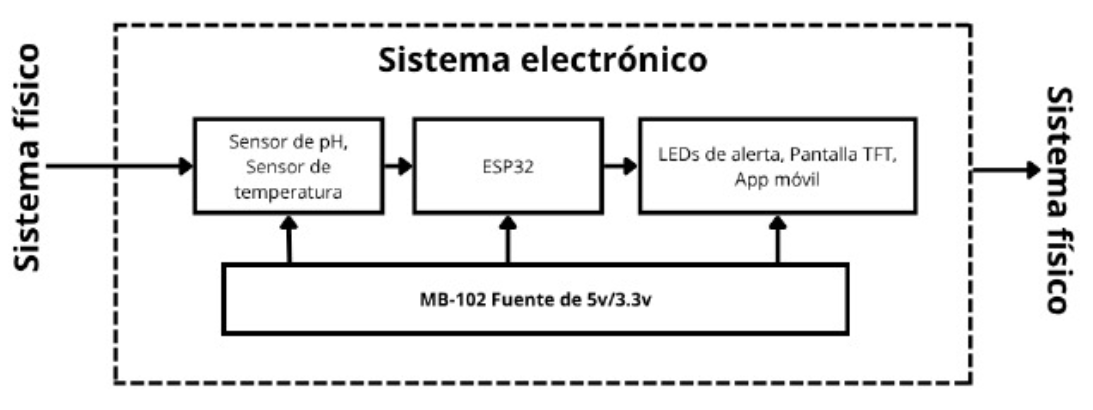
\includegraphics[width=0.9\textwidth]{diagrama.png}
				\caption{Diagrama de bloques del sistema de monitoreo HYDRAWARE}
				\label{fig:diagrama_bloques}
			\end{figure}
		\end{itemize}
		
		\subsubsection{Plataformas de Sistemas Embebidos}
		\begin{itemize}
			\item Identificar las plataformas de sistemas embebidos.
		\end{itemize}
		\subsubsection{Proceso de Selección de Plataformas}
		\begin{itemize}
			\item Explicar el proceso de selección de plataformas de sistemas embebidos de acuerdo a la función del proyecto.... Por que eliguieron una pagina web a una app movil.
		\end{itemize}
		\subsubsection{Proceso de Diseño y Construcción}
		\begin{itemize}
			\item Explicar el proceso de diseño de sistemas embebidos.
			\item Explicar el proceso de construcción de sistemas embebidos.
		\end{itemize}
		\subsubsection{Aplicaciones}
		\begin{itemize}
			\item Explicar las aplicaciones de microcontroladores en la robótica, domótica e internet de las cosas y como se integra en el proyecto... 
		\end{itemize}
	\end{itemize}
	
	
	\subsection{Descripción del proyecto a desarrollar}
	Automatizar procesos que, si se realizan de la manera antigua, resultan bastante tardados, es fundamental para mejorar la eficiencia operativa. Lo que se tiene pensado es aumentar la productividad y disminuir el tiempo estimado para medir parámetros críticos como el pH y la temperatura del agua en los estanques de cultivo. Actualmente, estas mediciones se llevan a cabo de forma manual, lo que representa una pérdida de tiempo y un riesgo para la salud de los peces debido a la falta de registros continuos y alertas tempranas ante desviaciones.
	
	Por esta razón, se propone el desarrollo HYDRAWARE, un sistema automatizado de monitoreo mediante el uso de sensores conectados a un microcontrolador y una aplicación móvil. Este sistema permitirá registrar, visualizar en tiempo real y generar alertas cuando los niveles de los parámetros se encuentren fuera de los límites aceptables, ya sea por valores bajos o elevados. Con esta solución tecnológica se busca mejorar la toma de decisiones, reducir errores humanos, optimizar el manejo del agua y promover una acuicultura más eficiente, precisa y sustentable.
	
	\subsection{Materiales}
	\begin{itemize}
		\item Sensor de Temperatura Digital Ds18b20.
		\item Adaptador para sensor Ds18b20
		\item PH-4502C
		\item Electrodo E201-BNC Tipo de sonda
		\item Display LCD 2x16
	\end{itemize}
	
	\subsection{Descripción de Arduino (ESP32-WROOM-32)}
	El ESP32-WROOM-32 es un módulo de microcontrolador (MCU) con conectividad Wi-Fi, Bluetooth y Bluetooth LE. Está diseñado para una variedad de aplicaciones, desde redes de sensores de baja potencia hasta tareas más exigentes como la codificación de voz y la transmisión de música. El núcleo del módulo es el chip ESP32-D0WDQ6.
	
	\subsubsection{Características principales:}
	\begin{itemize}
		\item \textbf{Conectividad Inalámbrica:}
		\begin{itemize}
			\item Wi-Fi: 802.11 b/g/n, con un rango de frecuencia central de 2412 a 2484 MHz.
			
			\item Bluetooth: Especificación v4.2 BR/EDR y Bluetooth LE. El receptor NZIF tiene una sensibilidad de -97 dBm, y el transmisor es Clase-1, Clase-2 y Clase-3.
		\end{itemize}
		
		\item \textbf{Interfaces del Módulo:}
		\begin{itemize}
			\item Soporta SD card, UART, SPI, SDIO, I2C, LED PWM, Motor PWM, I2S, IR, DAC, TWAI (compatible con CAN 2.0), sensor táctil capacitivo, ADC y contador de pulsos GPIO.
		\end{itemize}
		
		\item \textbf{Hardware Integrado:}
		\begin{itemize}
			\item Cristal de 40 MHz y Flash SPI de 4 MB.
		\end{itemize}
		
		\item \textbf{Condiciones de Operación:}
		\begin{itemize}
			\item Voltaje de operación: 3.0V 3.6V.
			\item Rango de temperatura: -40C +85C.
			\item Corriente de operación promedio: 80 mA.
		\end{itemize}
		\item \textbf{CPU y Memoria Interna:}
		\begin{itemize}
			\item Dos microprocesadores Xtensa® 32-bit LX6 de baja potencia.
			
			\item 520 KB de SRAM en chip, 448 KB de ROM para arranque y 16 KB de SRAM en RTC.
			
			
		\end{itemize}
	\end{itemize}
	
	\subsubsection{Elementos principales:}
	\begin{itemize}
		\item Módulo ESP32-WROOM-32.
		
		\item Chip ESP32-D0WDQ6.
		
		\item Conectividad Wi-Fi y Bluetooth/Bluetooth LE.
		
		\item Flash SPI de 4 MB y cristal oscilador de 40 MHz.
		
		\item Pines GPIO, con los GPIO6 a GPIO11 conectados a la flash SPI y no recomendados para otros usos.
		
		
	\end{itemize}
	
	\subsection{Software utilizado para la interfaz Usuario - Arduino}
	
	\subsection{Justificacion del Software Seleccionado}
	\subsection{Diagrama}
	A continuación se presenta un diagrama de bloques del sistema HYDROWARE, el cual representa los componentes principales y sus interconexiones para lograr el monitoreo automatizado.
	
	\begin{figure}[h]
		\centering
		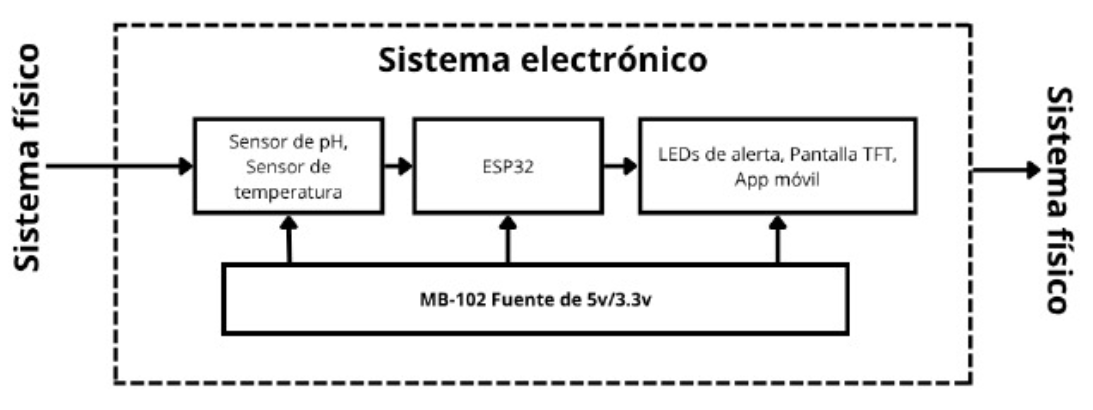
\includegraphics[width=0.9\textwidth]{diagrama.png}
		\caption{Diagrama de bloques del sistema de monitoreo HYDRAWARE}
		\label{fig:diagrama_bloques}
	\end{figure}



\end{document}